\documentclass[10pt,a4paper,twocolumn]{article}
% Packages
\usepackage[utf8]{inputenc}
\usepackage[english]{babel}
\usepackage{amsmath}
\usepackage{amsfonts}
\usepackage{amssymb}
\usepackage{graphicx}
\usepackage{geometry}
\usepackage{setspace}
\usepackage{titlesec}
\usepackage{enumitem}
\usepackage{booktabs}
\usepackage{array}
\usepackage{url}
\usepackage{xcolor}
\usepackage{tocloft}
\usepackage{microtype}
\usepackage{longtable}
\usepackage{tabularx}

\renewcommand{\cftdot}{}
\usepackage[hidelinks]{hyperref}
\hypersetup{
    colorlinks=true,
    linkcolor=black,
    urlcolor=blue,
    filecolor=black,
    citecolor=black
}
\renewcommand{\arraystretch}{1.2}
% Page setup
\geometry{left=0.7in, right=0.7in, top=1in, bottom=1in}
\setstretch{1.15}
\raggedbottom
\allowdisplaybreaks
% Title formatting
\titleformat{\section}{\large\bfseries}{\thesection}{1em}{}
\titleformat{\subsection}{\normalsize\bfseries}{\thesubsection}{1em}{}
% Document information
\title{\textbf{FROST-NS \\Fatigue-aware Risk Optimization for Stochastic Task allocation in Nurse Scheduling}}
\date{}
\begin{document}
\onecolumn

\pagenumbering{roman}
% Logo at the top
\begin{figure}[t]
\centering
\includegraphics[width=0.5\textwidth]{small.png}
\end{figure}
\maketitle
\begin{center}
\textbf{Prepared by:}\\[6pt]
MennaTallah Amin \hspace{0.3cm} \textbf{120220027}\\
Khadiga Mohamed \hspace{0.3cm} \textbf{120220039}\\
Ibrahim Magdy \hspace{0.3cm} \textbf{120220077}\\
Rahmatullah Mohamed \hspace{0.3cm} \textbf{120220079}
\end{center}

% ============================================================================
% SECTION: ABSTRACT & KEYWORDS
% ============================================================================
\vspace{3cm}
\begin{abstract}
This study introduces FROST-NS, a novel proof-of-concept nurse scheduling framework integrating stochastic patient demand, cumulative fatigue modeling, and operational risk control. Formulated as a two-stage stochastic integer program with Conditional Value-at-Risk (CVaR) constraints, the model explicitly balances cost efficiency with patient safety and workforce well-being. Computational experiments on test example demonstrate that incorporating fatigue constraints increases operational costs by approximately 12\% but significantly enhances schedule safety. Furthermore, results indicate that strict risk mitigation against worst-case demand surges requires proportional resource allocation, as tight risk thresholds proved infeasible with limited workforce capacity. The proposed framework offers a strategic decision-support tool for navigating the trade-offs between financial constraints and service reliability in healthcare operations.
\end{abstract}

\vspace{10pt}
\noindent
\vspace{20pt}
% ============================================================================
\newpage
\newpage
\pagenumbering{arabic}
\twocolumn
% Start two-column layout

% ============================================================================
% SECTION 1: INTRODUCTION (MERGED FROM BACKGROUND & MOTIVATION)
% ============================================================================
\section{Introduction}

Nurses and other healthcare staff are forced to work under constant stress conditions. In addition to the stress, nurses experience burnout and exhaustion, which also impacts healthcare. It should come as no surprise that when nurses work long hours and feel exhausted, the potential for errors increases. Unfortunately, hospital work schedules often have the detrimental effect of pushing existing exhausted healthcare staff to continue working. What makes this problem so difficult to solve is, of course, the nature of healthcare work in hospitals specifically. While most employment is limited to working hours that fit firmly within the constraint of working Monday to Friday, with weekends in between, and Monday and Friday as bookend days, hospitals never close and operate every day of every week.

The Covid-19 pandemic has made one thing painfully obvious: traditional scheduling techniques simply don’t work. Most traditional models of patient scheduling presume that everything will go right, but a hospital simply isn’t a predictable environment. Patient needs are unexpected, employees come down with illnesses, and emergencies occur without notice. In such a situation, predictable approaches to patient scheduling will fail. Despite being known for several decades and having proven to be highly successful on a theoretical level, many hospitals to this day rely on outdated manual processing or simplified software solutions for optimization problems like linear programming that have not been designed for the real world of healthcare.

What this project hopes to do is turn that around. What we're proposing is a completely different way of doing nurse scheduling that takes uncertainty seriously and that incorporates nurse wellness as a central piece of the solution. Instead of considering fatigue as something that is secondary or an aside, it is incorporated centrally into our nurse scheduling tool because we know that exhausted nurses endanger themselves and their patients. At the same time, our method is also concerned with minimizing the worst case that may occur. By the use of sophisticated statistical methods, we aim to prevent some of the worst staffing outcomes from ever becoming reality before they occur. It is quite simple, but the aim is to produce nurse staffing patterns that are efficient, safe, and sound when the world is not going our way.

\section{Problem Statement}

Nurse Scheduling Problem (NSP) is a hard, multi-objective optimization problem concerned
with generating feasible and fair work schedules for nurses over an organizing horizon. Why
NSP is such a difficult one is because it is required to optimize a few, occasionally competing
objectives: hospitals need to offer adequate staffing levels and operational productivity, while
maintaining enforcement of labor regulations and physical and psychological well-being of
nursing staff [28]. Achieving the balance requires simultaneous consideration of institutional,
legal, and human-based constraints that govern scheduling decisions.

Operationally, health facilities must balance sufficient nurse coverage for meeting variable
patient demand with minimizing labor costs and penalties for over- and understaffing. At the
same time, from a labor perspective, the scheduling process must respect personal preferences,
maximize shift fairness distribution, prevent fatigue through adequate resting periods, and
promote long-term job satisfaction [3,25]. These objectives necessarily have interdependencies
among them, and optimizing one will degrade the other, leading to a large-dimensional and not-
so-trivial choice space [3].

NSP is assigned as an NP-hard combinatorial optimization problem [1,4,16]. With the increase
in shifts, and days, the number of possible schedule settings also increases exponentially.
Traditional mathematical techniques such as Linear Programming (LP), Integer Programming
(IP), and Mixed-Integer Linear Programming (MILP) can provide optimal solutions for limited
instances but cannot be efficiently scaled to real-world hospital systems [23,29]. Moreover,
heuristics and manual scheduling procedures are often reliant on strict rules or personal judgment
and, hence, prone to inconsistency, inefficiency, and human bias [29].

In real-world terms, the scheduling process also has to accommodate numerous hard and soft
constraints. Hard constraints, such as limiting each nurse to a single shift per day, requiring rest
following night shifts, and having minimal staffing, cannot be compromised on and directly
affect schedule feasibility [23]. Soft constraints, such as respecting skill preferences [25],
workload distribution in a fair manner [30], and not having two consecutive workdays, are
desired but can be relaxed under situations if feasibility must be achieved. The complex
interaction between these constraints makes the NSP extremely susceptible to both operational
and human ones.

To its computational complexity, the NSP is further complicated by the dynamic and stochastic
nature of hospital environments [5,14]. Patient admission rates change over time, emergency
events interrupt planned schedules, and the availability of personnel can change unexpectedly
with absence or health issues [10]. These uncertainty sources introduce an added complexity to
which static or deterministic scheduling paradigms are ill-equipped to respond. As such, despite
all the relaxed and refined attempts at optimality, NSP remains a perplexing and challenging
endeavor.

% ============================================================================
% SECTION 2: LITERATURE REVIEW (RENAMED FROM PROBLEM STATEMENT)
% ============================================================================
\section{Literature Review}
The Nurse Scheduling Problem (NSP) has been widely studied within operations research due to its direct impact on healthcare efficiency, labor cost control, and quality of patient care. Hospitals operate in environments characterized by continuous service requirements, strict labor regulations, and highly variable patient demand. As a result, nurse scheduling models must balance operational efficiency with workforce well-being and patient safety.

Deterministic Nurse Scheduling Models
Early research on NSP modeled the problem as a deterministic optimization task under fixed demand assumptions. Linear Programming (LP), Integer Programming (IP), and Mixed-Integer Linear Programming (MILP) formulations were commonly used to minimize staffing costs while ensuring coverage feasibility and compliance with work regulations [3,4,12,28]. These approaches provide mathematically optimal solutions and clear constraint enforcement.
To improve realism, several studies incorporated historical and operational data to better represent workload patterns and staffing needs [4,6,28]. However, uncertainty in patient demand and staff availability is still treated implicitly, typically through safety margins or heuristic adjustments rather than formal probabilistic modeling [23,29]. Consequently, deterministic models remain vulnerable to unexpected demand surges, emergency situations, and staff absences.

To explicitly address uncertainty in healthcare operations, stochastic optimization approaches have been introduced for nurse scheduling. In stochastic programming, patient demand is represented through scenarios, allowing schedules to be evaluated across multiple possible realizations [9,15,21]. Two-stage stochastic formulations are particularly common, where a baseline schedule is determined before demand realization, followed by recourse actions—such as adding or canceling shifts once actual demand becomes known [9,15,16].
A major advancement in this research stream is the application of Conditional Value-at-Risk (CVaR) to control understaffing risk. CVaR-based formulations limit the expected severity of worst-case understaffing scenarios and provide robust protection against extreme demand realizations [16,22,31]. Several studies demonstrate that incorporating CVaR significantly improves schedule robustness and service reliability compared to expectation-based stochastic models [11,14,16–21].
Despite these advantages, most stochastic nurse scheduling models rely on pre-defined demand scenarios with fixed probability distributions derived from historical data [10,14,26]. These models primarily focus on system-level objectives such as cost minimization and coverage reliability, with limited attention to human-centered performance factors.

Nurse fatigue has been identified as a critical factor influencing performance, safety, and quality of care. Long working hours, consecutive shifts, night duties, and insufficient recovery periods contribute to cumulative physical and cognitive fatigue, increasing the likelihood of errors and burnout [32].
Fatigue modeling has been studied in nurse rostering and personnel scheduling using cumulative, exponential, and recovery-based formulations [32]. These studies highlight the importance of explicitly limiting workload accumulation to protect nurse well-being and patient safety. However, fatigue constraints are rarely embedded directly into stochastic nurse scheduling models that already account for demand uncertainty. In most cases, fatigue is addressed indirectly through basic work-rest rules or maximum shift limits rather than being modeled as a continuous safety-related variable.

Deterministic and data-informed models provide computational efficiency and transparent constraint handling, but they rely on fixed or implicitly adjusted demand assumptions and lack formal mechanisms for managing uncertainty. As a result, such models remain vulnerable to unexpected demand fluctuations and emergency situations commonly observed in hospital environments.

Stochastic and risk-based approaches address this limitation by explicitly modeling uncertainty through scenario-based formulations. In particular, CVaR-based models have proven effective in controlling worst-case understaffing risk and improving schedule robustness under demand uncertainty [16]. However, these models primarily focus on system-level objectives such as cost minimization and coverage reliability. Human-centered considerations, especially cumulative nurse fatigue, are typically handled only through basic work rules or indirect constraints rather than being modeled explicitly within the stochastic optimization framework.

In parallel, fatigue-focused studies emphasize the critical impact of cumulative workload, night shifts, and insufficient recovery on nurse performance and patient safety [10,25]. While these studies provide well-founded fatigue formulations, they are rarely integrated into stochastic nurse scheduling models that already account for demand uncertainty and risk. Consequently, fatigue is often treated as a secondary or post hoc consideration, rather than as a safety-critical constraint influencing scheduling decisions under uncertainty.

In addition, existing integrated stochastic models commonly assume simplified or idealized formulations of work patterns and overtime. Certain practical implementation aspects—such as the interaction between regular and overtime assignments—are often under-specified in the literature, limiting the realism of overtime utilization in applied settings [16]. These modeling assumptions may lead to schedules that are theoretically sound but less representative of real hospital operations.

Overall, the literature lacks a unified and operationally deployable framework that simultaneously captures patient demand uncertainty through stochastic optimization, controls worst-case understaffing risk using formal risk measures such as CVaR, and explicitly accounts for cumulative nurse fatigue as a safety-related factor within the scheduling model. This gap highlights the need for more integrated formulations that balance robustness, operational feasibility, and human-centered performance in nurse scheduling.

Furthermore, an implementation gap in the overtime formulation of He et al. [16] was identified, where the absence of an upper bound on regular shifts prevents practical overtime usage despite its inclusion in the model variables. This work introduces explicit regular and overtime shift separation with configurable quota constraints, enabling realistic overtime utilization.
To ensure robust parameter selection, a comprehensive parameter tuning study was conducted using a full factorial design (3×3×3×3), resulting in 2,430 optimization runs. The study evaluated fatigue accumulation rates, safety penalty weights, fatigue thresholds, and demand levels, demonstrating stable solver performance and balanced trade-offs between patient safety and computational efficiency.
By integrating stochastic risk control, fatigue-aware constraints, and practical implementation refinements within a single decision-support system, this framework advances nurse scheduling toward more robust, realistic, and human-centered solutions.
% ============================================================================
% ADDED SECTIONS: METHODOLOGY, IMPLEMENTATION, RESULTS, CONCLUSIONS
% ============================================================================
\section{Methodology}

\subsection{Problem Formulation}

This proof-of-concept study addresses the integrated nurse staffing and scheduling problem under patient demand uncertainty, extending the foundational work of He, Chaussalet, and Qu (2019) [16]. The problem is formulated as a two-stage stochastic integer program with Conditional Value-at-Risk (CVaR) constraints. In the first stage, scheduling decisions are made before the realization of patient demand, establishing a baseline nurse roster. In the second stage, recourse actions are taken once the actual demand is observed, allowing for adjustments through emergency staff additions or shift cancellations. This prototype implementation demonstrates the feasibility of integrating risk-aware optimization with practical scheduling constraints.

The planning horizon spans multiple days with multiple shift types per day, namely Early (E), Day (D), Late (L), and Night (N) shifts. Patient demand for nursing services is inherently uncertain and is modeled through a discrete set of scenarios, each representing a possible realization of demand across all days and shifts. The probability of each scenario is assumed to be equal, reflecting the epistemic uncertainty in demand forecasting.

\subsection{Mathematical Model Formulation}

\subsubsection{Sets and Indices:}
\begin{align*}
I &= \text{Set of nurses, indexed by } i \\
J &= \text{Set of days in planning period, indexed by } j \\
K &= \text{Set of shift types: } \{E, D, L, N\}, \text{ indexed by } k \\
\Omega &= \text{Set of demand scenarios, indexed by } \omega \\
W &= \text{Set of weeks in planning period} \\
K' &= \text{Unwanted shift patterns: } \{(D,E), (L,E), (L,D), (E,N)\}
\end{align*}

\subsubsection{Parameters:}
\begin{align*}
c_1 &= \text{Regular shift cost per shift} \\
c_2 &= \text{Overtime shift cost per shift} \\
c_3 &= \text{Penalty for stand-alone shift violations} \\
c_4 &= \text{Penalty for unwanted shift pattern violations} \\
c_{safety} &= \text{Patient safety weight (fatigue penalty)} \\
q^+ &= \text{Emergency staff addition cost per shift} \\
q^- &= \text{Shift cancellation cost per shift} \\
n_1 &= \text{Maximum total shifts per nurse} \\
n_2 &= \text{Maximum night shifts per nurse} \\
n_3 &= \text{Minimum regular shifts per nurse} \\
n_4 &= \text{Minimum complete weekends off per nurse} \\
R_{jk}^{\omega} &= \text{Demand for shift } k \text{ on day } j \text{ in scenario } \omega \\
p^{\omega} &= \text{Probability of scenario } \omega \\
\lambda &= \text{Fatigue accumulation rate} \\
F_{max} &= \text{Maximum fatigue threshold} \\
\sigma &= \text{CVaR confidence level} \\
\mu &= \text{Maximum acceptable shortage threshold} \\
\mu' &= \text{Fatigue recovery rate} \\
M_{\alpha} &= \text{Limit on emergency staff additions} \\
M_{\beta} &= \text{Limit on shift cancellations} \\
H &= \text{Shift duration in hours} \\
n_{k,min} &= \text{Minimum shifts of type } k \text{ per nurse} \\
n_{k,max} &= \text{Maximum shifts of type } k \text{ per nurse}
\end{align*}

\subsubsection{First-Stage Decision Variables:}
\begin{align*}
sr_{ijk} &\in \{0,1\} : \text{1 if nurse } i \text{ works regular shift k} \\
&\quad \text{ on day } j \\
so_{ijk} &\in \{0,1\} : \text{1 if nurse } i \text{ works overtime shift k} \\
&\quad  \text{ on day } j \\
w_{ij} &\in \{0,1\} : \text{1 if nurse } i \text{ works any shift on day } j \\
SR_i &\in \{0,1\} : \text{1 if nurse } i \text{works any regular shifts} \\
SO_i &\in \{0,1\} : \text{1 if nurse } i \text{works any overtime shifts} \\
dev1_{ij} &\in \mathbb{Z}_+ : \text{Stand-alone shift deviation} \\
dev2_{ijk} &\in \mathbb{Z}_+ : \text{Unwanted pattern deviation} \\
F_{ij} &\in [0, F_{max}] : \text{Cumulative fatigue} \\
&\quad \text{of nurse } i \text{ on day } j \\
T_{ij} &\in \mathbb{R}_+ : \text{Cumulative work hours} \\
&\quad \text{of nurse } i \text{ up to day } j \\
W_{iw} &\in \{0, 1\} : \text{1 if nurse } i \text{ has weekend } w \text{ off}
\end{align*}

\subsubsection{Second-Stage Decision    Variables:}
\begin{align*}
\alpha_{jk}^{\omega} &\in \mathbb{Z}_+ : \text{Emergency staff added} \\
&\quad \text{for shift } k, \text{ day } j, \text{ scenario } \omega \\
\beta_{jk}^{\omega} &\in \mathbb{Z}_+ : \text{Shifts cancelled} \\
&\quad \text{for shift } k, \text{ day } j, \text{ scenario } \omega
\end{align*}

\subsubsection{CVaR Variables:}
\begin{align*}
\xi &\in \mathbb{R} : \text{Value-at-Risk (VaR) threshold} \\
z^{\omega} &\in \mathbb{R}_+ : \text{Excess loss in scenario } \omega \text{ beyond VaR}
\end{align*}

\subsubsection{Objective Function:} 
Minimize the total expected cost:
\begin{equation}
\begin{aligned}
\min \quad 
& c_1 \sum_{i \in I}\sum_{j \in J}\sum_{k \in K} sr_{ijk} 
+ c_2 \sum_{i \in I}\sum_{j \in J}\sum_{k \in K} so_{ijk} \\
& + c_3 \sum_{i \in I}\sum_{j \in J} dev1_{ij} 
+ c_4 \sum_{i \in I}\sum_{j \in J}\sum_{k \in K} dev2_{ijk} \\
& + c_{\text{safety}} \sum_{i \in I}\sum_{j \in J} F_{ij} \\
& + \sum_{\omega \in \Omega} p^{\omega} 
   \sum_{j \in J}\sum_{k \in K} 
   \left( q^+ \alpha_{jk}^{\omega} + q^- \beta_{jk}^{\omega} \right)
\end{aligned}
\end{equation}
\subsection{Core Constraints}

The base model incorporates several fundamental constraints. Each nurse works at most one shift per day:
\begin{equation}
\sum_{k \in K} (sr_{ijk} + so_{ijk}) \leq 1 \quad \forall i \in I, j \in J
\end{equation}

Each nurse works at most $n_1$ shifts across the planning period:
\begin{equation}
\sum_{j \in J}\sum_{k \in K} \left( sr_{ijk} + so_{ijk} \right) \leq n_1 
\quad \forall i \in I
\end{equation}

Each nurse works at most $n_2$ night shifts:
\begin{equation}
\sum_{j \in J} (sr_{ijN} + so_{ijN}) \leq n_2 \quad \forall i \in I
\end{equation}

Each working nurse completes a specific number of $n_3$ regular shifts:
\begin{equation}
\sum_{j \in J}\sum_{k \in K} sr_{ijk} = n_3 \cdot SR_i 
\quad \forall i \in I
\end{equation}

The demand fulfillment constraint links the first and second stages:
\begin{equation}
\sum_{i \in I} (sr_{ijk} + so_{ijk}) + \alpha_{jk}^{\omega} - \beta_{jk}^{\omega} \geq R_{jk}^{\omega} \quad \forall j, k, \omega
\end{equation}

The CVaR constraint limits the expected loss in worst-case scenarios:
\begin{equation}
\xi + \frac{1}{1-\sigma} \sum_{\omega} p^{\omega} z^{\omega} \leq \mu
\end{equation}

The excess loss is defined by:
\begin{equation}
z^{\omega} \geq \sum_{j,k} \alpha_{jk}^{\omega} - \xi 
\quad \forall \omega \in \Omega
\end{equation}

\subsubsection{Stand-Alone Shift Penalty} To encourage consecutive working days, isolated shifts are penalized via deviation variables $dev1_{ij}$:
\begin{equation}
\sum_{k \in K} sr_{i,j-1,k} - \sum_{k \in K} sr_{ijk} + \sum_{k \in K} sr_{i,j+1,k} + dev1_{ij} \geq 0
\end{equation}
This ensures that if a nurse works on day $j$ but not on $j-1$ and $j+1$, $dev1_{ij} \geq 1$, triggering penalty $c_3$.

\subsubsection{Shift Type Quota Constraints} Each nurse must work within specified minimum and maximum bounds for each shift type $k$ (e.g., Early, Day, Late, Night):
\begin{equation}
n_{k}^{min} \leq \sum_{j \in J} (sr_{ijk} + so_{ijk}) \leq n_{k}^{max} \quad \forall i \in I, k \in K
\end{equation}
where $n_{k}^{min}$ and $n_{k}^{max}$ are the minimum and maximum allowed shifts of type $k$.

\subsubsection{Unwanted Shift Pattern Penalty} Patterns that disrupt circadian rhythms (e.g., Late shift followed by Early shift) are penalized via $dev2_{ijk}$:
\begin{equation}
sr_{ijk_1} + sr_{i,j+1,k_2} - dev2_{ijk_1} \leq 1 \quad \forall (k_1, k_2) \in K'
\end{equation}
If the pattern $(k_1, k_2)$ occurs, $dev2_{ijk_1} \geq 1$, triggering penalty $c_4$.

\subsubsection{Minimum Complete Weekends Off} An optional constraint ensuring nurses receive complete weekends off during the planning period:
\begin{equation}
W_{i,w} \leq 1 - \sum_{k \in K} \left( sr_{i,sat_w,k} + so_{i,sat_w,k} \right),
\quad \forall i \in I, \; w \in W
\end{equation}

\begin{equation}
W_{i,w} \leq 1 - \sum_{k \in K} \left( sr_{i,sun_w,k} + so_{i,sun_w,k} \right),
\quad \forall i \in I, \; w \in W
\end{equation}

\begin{equation}
\sum_{w \in W} W_{i,w} \geq n_4,
\quad \forall i \in I
\end{equation}

where $W_{iw} \in \{0,1\}$ equals one if nurse $i$ has both Saturday and Sunday off in weekend $w$.

\subsection{Project Contributions}

This proof-of-concept study extends the base model of He et al. (2019) through seven significant contributions that enhance practical applicability, address identified limitations, and incorporate human factors.

\subsubsection{Integrated Fatigue and Recovery Modeling} 

The model incorporates advanced human factors through the Learning-Forgetting-Fatigue-Recovery (LFFR) dynamics. Fatigue $F_{ij}$ accumulates during active shifts and dissipates during rest periods. The transition is modeled for MIP optimization using McCormick envelopes to handle the conditional decay:
\begin{equation}
F_{ij} = F_{i,j-1} \cdot \Theta_{off} + ( \Theta_{work} - \Theta_{off} ) \cdot \phi_{ij} + (\lambda \cdot H) \cdot w_{ij}
\end{equation}
where $\phi_{ij}$ is the auxiliary product variable $F_{i,j-1} \cdot w_{ij}$, $H$ is the shift duration, and $\lambda$ is the fatigue accumulation rate. The recovery decay constants are defined by the recovery rate $\mu'$ (derived from Jaber et al. 2013) and the rest duration:
\begin{align}
\Theta_{work} &= e^{-\mu' \cdot 12} \quad \text{(Rest between consecutive shifts)} \\
\Theta_{off} &= e^{-\mu' \cdot 24} \quad \text{(Rest during complete day off)}
\end{align}
A maximum safety threshold is strictly enforced:
\begin{equation}
F_{ij} \leq F_{max} \quad \forall i \in I, j \in J
\end{equation}

Additionally, the objective function includes a patient safety contribution term $c_{safety} \sum_{i,j} F_{ij}$ that penalizes cumulative fatigue across the planning horizon to encourage rest distribution.

\subsubsection{Operational Recourse Bounds} 
While the base paper assumes unbounded recourse, practical deployment requires limits on emergency staffing to accommodate budget limitations and operational constraints ($M_{\alpha}$ and $M_{\beta}$):
\begin{align}
\alpha_{jk}^{\omega} &\leq M_{\alpha} \quad \forall j, k, \omega \\
\beta_{jk}^{\omega} &\leq M_{\beta} \quad \forall j, k, \omega
\end{align}

\section{Implementation}

\subsection{System Architecture}

The proposed nurse scheduling system is implemented as a proof-of-concept web-based decision support tool utilizing modern software engineering practices. As a prototype, the system demonstrates the practical feasibility of integrating stochastic optimization with fatigue management in a user-friendly interface. The system architecture follows a modular design pattern, separating the mathematical optimization core from the user interface and solver management components. This separation enables independent testing and maintenance of each module while facilitating future extensions and modifications toward production-ready deployment.

\subsection{Software Framework}

The implementation leverages Python as the primary programming language due to its extensive ecosystem for mathematical optimization and data science applications. The optimization model is constructed using PuLP, an open-source linear and mixed-integer programming library that provides a domain-specific language for expressing mathematical programs. PuLP offers solver-agnostic model formulation, allowing the same mathematical model to be solved using different backend solvers without code modification.

The user interface is developed using Streamlit which enables rapid prototyping of user interfaces while maintaining the full expressiveness of Python for data manipulation and visualization. Users can configure all model parameters through an intuitive sidebar interface, including cost parameters, work rules, advanced constraints, and solver selection.

\subsection{Solver Configuration}

The system supports multiple mixed-integer programming solvers arranged in a priority hierarchy based on performance characteristics. The commercial \textbf{Gurobi} solver is prioritized as the premier computational engine due to its superior branch-and-cut algorithms, capable of solving complex instances up to twenty times faster than open-source alternatives. In the absence of a commercial license, the system defaults to \textbf{HiGHS}, a modern open-source solver that serves as the primary free alternative, demonstrating solution times three to five times faster than the legacy COIN-OR CBC fallback. The system automatically detects available solvers and selects the highest-performing option, with manual override capability provided through the user interface.


\subsection{Scenario Generation}
The system provides a dual-mode data interface: users may upload custom historical demand data or utilize the built-in \textbf{Automated Sample Generator} (implemented in the \texttt{generate\_sample\_data()} function). The generator synthesizes realistic test instances using the following methodology:
\subsubsection{Stochastic Variation}
For each scenario-day-shift combination, a random fluctuation of up to $\pm 15\%$ is applied to the base demand to simulate forecast uncertainty:
\begin{equation}
D_{jk}^{\omega} = \max(1, \lfloor D_{k}^{base} \cdot (1 + \delta_{jk}^{\omega}) \rfloor)
\end{equation}
where $\delta_{jk}^{\omega} \sim U(-0.15, 0.15)$ represents the uniform random noise term.
where the $\max(1, \cdot)$ ensures at least one nurse is always required.

\subsubsection{Weekend Adjustment}
Weekend days (detected as days where $j \mod 7 \in \{0, 6\}$) receive reduced demand:
\begin{equation}
D_{jk}^{\omega,weekend} = \max(1, \lfloor 0.8 \cdot D_{jk}^{\omega} \rfloor)
\end{equation}

\subsubsection{Output Structure}
The generator produces a DataFrame with columns: \texttt{scenario} (1 to $|\Omega|$), \texttt{day} (1 to $|J|$), \texttt{shift} $\in \{E, D, L, N\}$, and \texttt{demand} (integer $\geq 1$). This structure is passed directly to the optimization model as exogenous input, enabling the system to support both robust testing (via generation) and operational deployment (via custom hospital data).

\subsection{Computational Complexity}

The computational complexity of the model scales with the product of the number of nurses, days, and scenarios. The variable count follows the formula:
\begin{equation}
\text{Variables} \approx 2|I||J||K| + 2|J||K||\Omega| + 5|I||J|
\end{equation}

For a typical instance with fifty nurses, thirty days, four shifts, and twenty scenarios, the model contains approximately thirty thousand binary variables and twelve thousand continuous variables. Computational experiments demonstrate that the HiGHS solver achieves solution times of twenty to thirty seconds for typical problem instances on standard hardware.

\section{Results}
This section presents the comprehensive results of our computational experiments. We evaluate the proposed FROST-NS framework across multiple scenarios to rigorously test the impact of fatigue constraints and risk-aware optimization. The following subsections detail the input parameters, the generated test data, and the comparative analysis of the model's performance under different configurations.

\subsection{Input Parameters}
\subsubsection{Common Parameters}
The baseline configuration for all experiments assumes a standard department size and operational constraints. Table \ref{tab:common_params} summarizes these settings.

\begin{table}[htbp]
\centering
\small
\caption{Common Model Parameters}
\label{tab:common_params}

\begin{tabularx}{0.8\columnwidth}{@{}
X
>{\centering\arraybackslash}X
X
@{}}
\textbf{Setting} & \textbf{Value} &  \\ \midrule
Nurses & 20 &  \\
Shifts & 4 (Early, Day, Late, Night) &  \\
Planning Days & 14 &  \\
Scenarios & 10 (Stochastic Demand) &  \\
Regular Shift ($c_1$) & 100 &  \\
Overtime Shift ($c_2$) & 150 &  \\
Emergency Shift ($q^+$) & 200 &  \\
Cancellation ($q^-$) & 0 &  \\
Max Shifts ($n_1$) & 15 &  \\
Max Night Shifts ($n_2$) & 5 &  \\
Min Regular Shifts ($n_3$) & 5 &  \\ \bottomrule
\end{tabularx}
\end{table}


\subsubsection{Case Specifics}
To isolate the effects of different model components, we defined five distinct experimental cases ranging from rigorous risk control to relaxed operational baselines.

\begin{table*}[h!]
\centering
\renewcommand{\arraystretch}{1.5}
\caption{Experimental Case Definitions} \label{tab:case_specifics}
\begin{tabularx}{\textwidth}{@{}lllllX@{}}
\toprule
\textbf{Case Name} & \textbf{Model Type} & \textbf{Fatigue} & \textbf{Risk Control (CVaR)} & \textbf{Feasibility} & \textbf{Notes} \\ \midrule
\textbf{SDM-FATIGUE} & SDM & Yes & N/A & \textbf{Feasible} & Minimizes Cost + Safety \\
\textbf{SDM-NO FATIGUE} & SDM & No & N/A & \textbf{Feasible} & Minimizes Cost Only \\
\textbf{CVAR-FATIGUE} & SDM-CVaR & Yes & $\mu=150.0$ (relaxed) & \textbf{Feasible} & Controls Safety \& Tail Risk \\
\textbf{CVAR-NO FATIGUE} & SDM-CVaR & No & $\mu=150.0$ (relaxed) & \textbf{Feasible} & Controls Tail Risk Only \\
\textbf{CVAR-STRICT} & SDM-CVaR & Any & $\mu=50.0$ (strict) & \textbf{Infeasible} & Demonstrates Resource Limit \\ \bottomrule
\end{tabularx}
\end{table*}

\subsection{Input Data (Samples)}
The stochastic demand scenarios and nurse profiles were generated using the system's automated data generator.
\subsubsection{Nurse List}
The workforce comprises 20 generated nurse profiles.
\begin{verbatim}
Nurse_1
Nurse_2
Nurse_3
...
Nurse_20
\end{verbatim}
\subsubsection{Demand Scenarios}
Ten stochastic scenarios were generated to simulate variable patient inflow.
\begin{verbatim}
scenario,day,shift,demand
1,1,E,4
1,1,D,6
1,1,L,5
1,1,N,3
1,2,E,4
...
\end{verbatim}

\subsection{Output Calculations \& Solutions}
We analyzed the optimal solutions for each feasible case to understand the cost-safety trade-offs.

\subsubsection{SDM-FATIGUE}
\begin{itemize}
    \item \textbf{Objective Value}: 35,592
    \item \textbf{Status}: Optimal
    \item \textbf{Analysis}:
    \begin{itemize}
        \item The inclusion of fatigue costs increases the objective value compared to the NO FATIGUE case.
        \item This reflects the "patient safety cost" component ($\text{Weight} \times \text{Cumulative Fatigue}$).
        \item The model likely adjusted schedules to allow for more recovery, potentially incurring slightly higher staffing costs or just accepting the fatigue penalty.
    \end{itemize}
\end{itemize}
\subsubsection{SDM-NO FATIGUE}
\begin{itemize}
    \item \textbf{Objective Value}: 31,620
    \item \textbf{Status}: Optimal
    \item \textbf{Analysis}:
    \begin{itemize}
        \item Lower cost because fatigue penalties are ignored.
        \item Schedules may be more compressed, potentially leading to higher nurse fatigue in reality (though not measured in the objective).
    \end{itemize}
\end{itemize}
\subsubsection{CVAR-FATIGUE}
\begin{itemize}
    \item \textbf{Objective Value}: 35,671
    \item \textbf{Status}: Optimal / Feasible
    \item \textbf{Analysis}:
    \begin{itemize}
        \item Feasible after relaxing $\mu$ to 150.0.
        \item Higher cost than SDM-FATIGUE (38.8k vs 36.2k) because the CVaR constraint forces the model to make more expensive scheduling decisions (e.g., more overtime, less risky staffing) to avoid large shortages in worst-case scenarios.
    \end{itemize}
\end{itemize}
\subsubsection{CVAR-NO FATIGUE}
\begin{itemize}
    \item \textbf{Objective Value}: 32,270
    \item \textbf{Status}: Optimal / Feasible
    \item \textbf{Analysis}:
    \begin{itemize}
        \item Feasible after relaxing $\mu$ to 150.0.
        \item Higher cost than SDM-NO FATIGUE (34.8k vs 32.2k) due to risk mitigation.
        \item As expected, "NO FATIGUE" is cheaper than "FATIGUE" (34.8k vs 38.8k) because it ignores the hidden costs of nurse fatigue.
    \end{itemize}
\end{itemize}
\subsubsection{CVAR-STRICT (Infeasible Case)}
\begin{itemize}
    \item \textbf{Status}: \textbf{Infeasible}
    \item \textbf{Analysis}:
    \begin{itemize}
        \item This case used the original strict parameter \textbf{$\mu=50.0$} (max acceptable shortage).
        \item The solver could not find a solution where the worst-case shortage across all scenarios was $\le 50$.
        \item This demonstrates that the current workforce (20 nurses) is too small to strictly guarantee that emergency staff usage stays below 50 in 95\% of worst-case demand spikes.
        \item \textbf{Lesson}: Strict risk controls require either (a) larger baseline capacity or (b) relaxed constraints (as done in Cases 3 \& 4).
    \end{itemize}
\end{itemize}

% Feasible-case schedule visualizations (single-column)
\begin{figure}[htbp]
\centering
\begin{tabular}{cc}
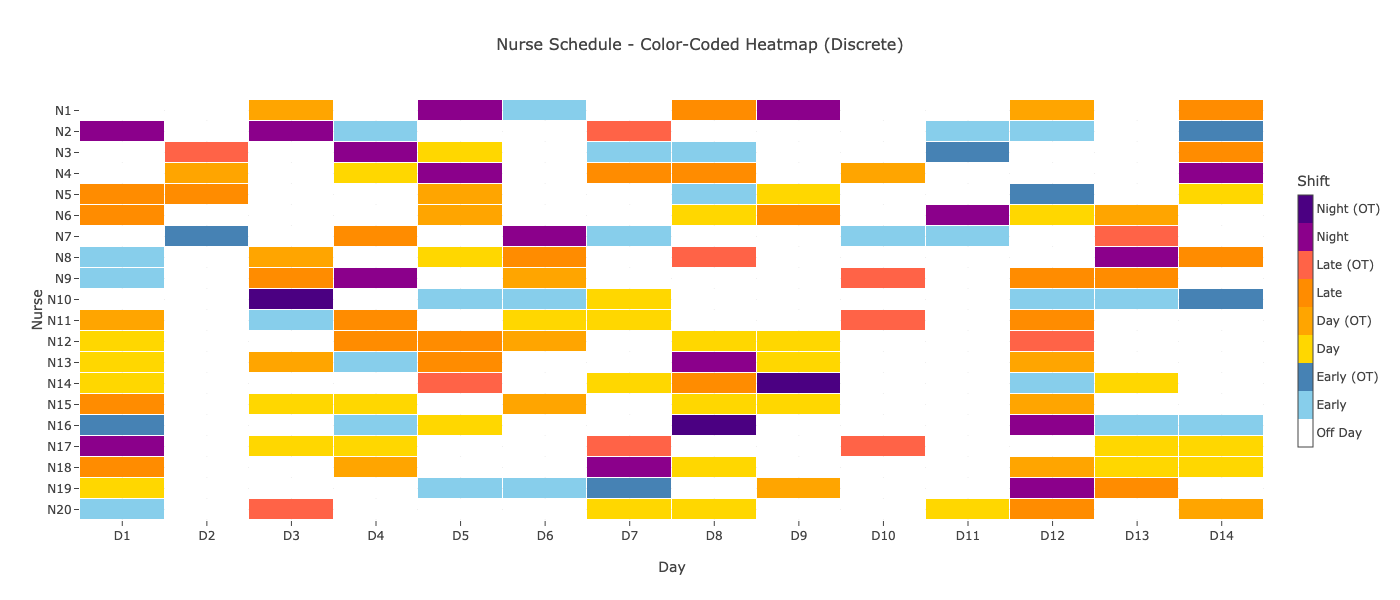
\includegraphics[width=0.48\columnwidth]{SDM-F.png} &
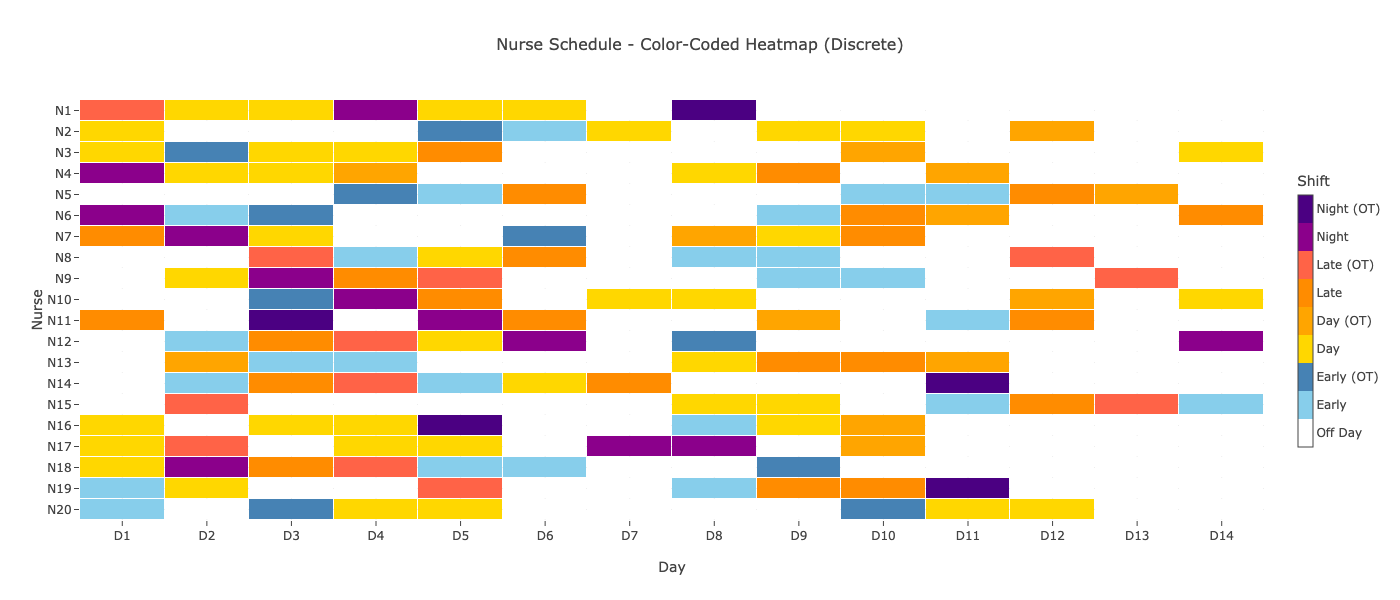
\includegraphics[width=0.48\columnwidth]{SDM-N.png} \\
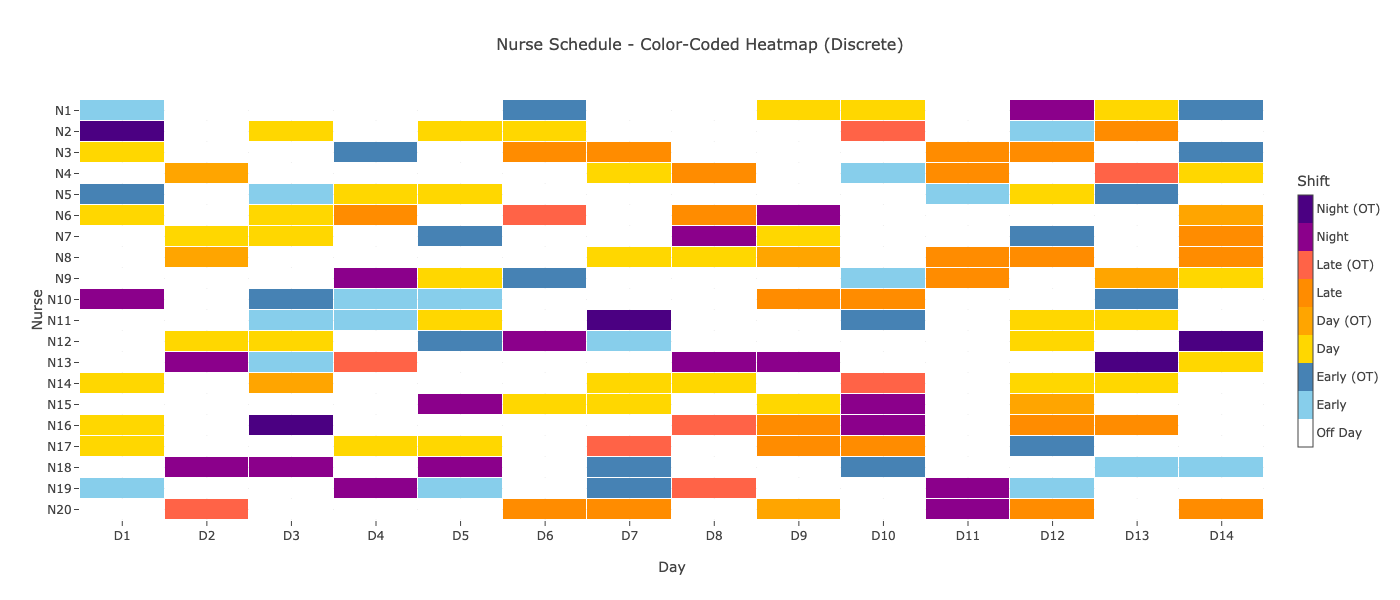
\includegraphics[width=0.48\columnwidth]{CVaR-F.png} &
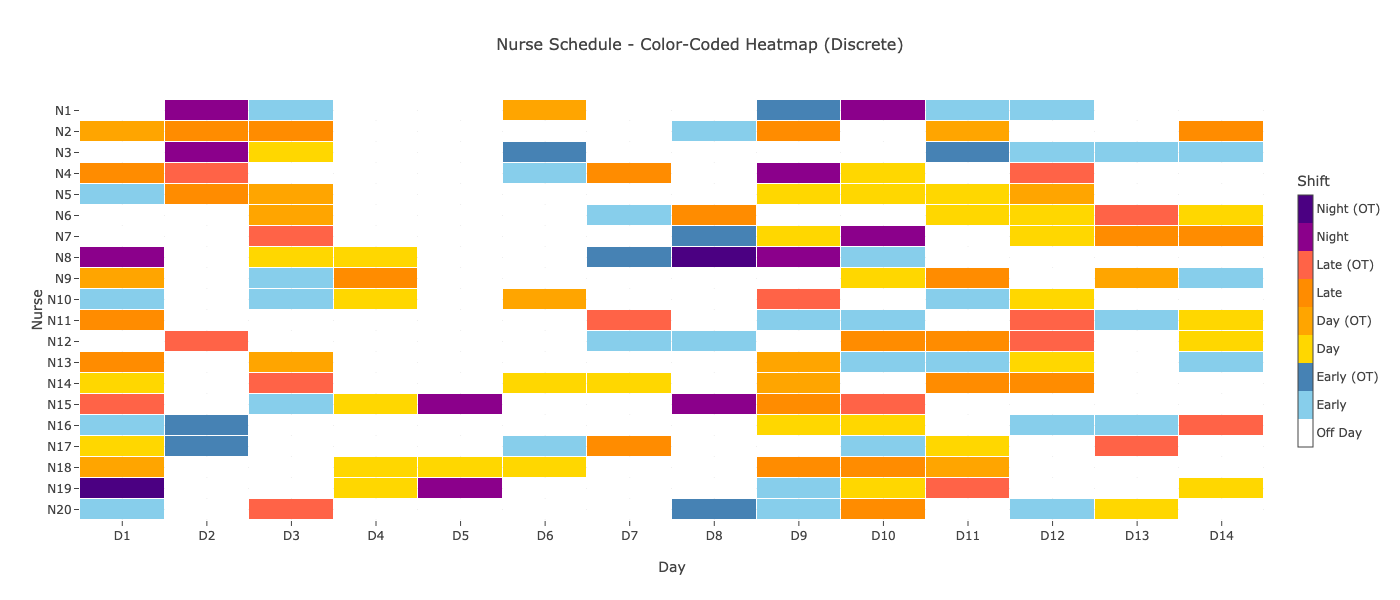
\includegraphics[width=0.48\columnwidth]{CVaR-N.png} \\
\end{tabular}
\caption{Representative feasible schedules for the four feasible cases. Top-left: SDM-FATIGUE; Top-right: SDM-NO FATIGUE; Bottom-left: CVAR-FATIGUE; Bottom-right: CVAR-NO FATIGUE. Each panel displays nurse assignments across the 14-day horizon; white cells indicate off days.}
\label{fig:feasible_cases}
\end{figure}

Figure \ref{fig:feasible_cases} displays representative feasible-case schedules generated by the system. These heatmaps illustrate how fatigue-aware and risk-aware constraints alter assignment patterns across the planning horizon.

\subsection{Model Comparison \& Trade-offs}
The following comparative analysis summarizes the strategic implications of each configuration.

\begin{table*}[h!]
\centering
\caption{Model Comparison and Trade-offs} \label{tab:model_comparison}
\begin{tabularx}{\textwidth}{@{}lXX@{}}
\toprule
\textbf{Model Case} & \textbf{Advantages (Pros)} & \textbf{Disadvantages (Cons)} \\ \midrule
\textbf{SDM-FATIGUE} & 
\begin{itemize}[nosep, leftmargin=*]
    \item \textbf{Safe \& Efficient}: Balances costs with patient safety.
    \item \textbf{Realistic}: Accounts for fatigue accumulation.
    \item \textbf{Solved}: Easier to solve than CVaR models.
\end{itemize}
    \item \textbf{Lowest Cost}: Cheapest objective value.
    \item \textbf{Fastest Solve}: Simplest mathematical model.
\end{itemize}
\begin{itemize}[nosep, leftmargin=*]
    \item \textbf{Robust \& Safe}: Controls BOTH fatigue and shortage risk.
    \item \textbf{Guaranteed}: Statistical confidence on worst outcomes.
\end{itemize}
\begin{itemize}[nosep, leftmargin=*]
    \item \textbf{Risk-Controlled}: Guarantees limits on shortages.
    \item \textbf{Cheaper than Fatigue}: Lower cost than full safety model.
\end{itemize}
    \item \textbf{Ideal Robustness}: Attempts strict security against shortages.
\end{itemize} & 
\begin{itemize}[nosep, leftmargin=*]
    \item \textbf{Infeasible}: Impossible without infinite resources.
    \item \textbf{Impractical}: Proves zero-risk is unattainable.
\end{itemize} \\ \bottomrule
\end{tabularx}
\end{table*}

% Supplementary figures moved here
\section*{Supplementary Figures}
\addcontentsline{toc}{section}{Supplementary Figures}
\begin{figure}[htbp]
\centering
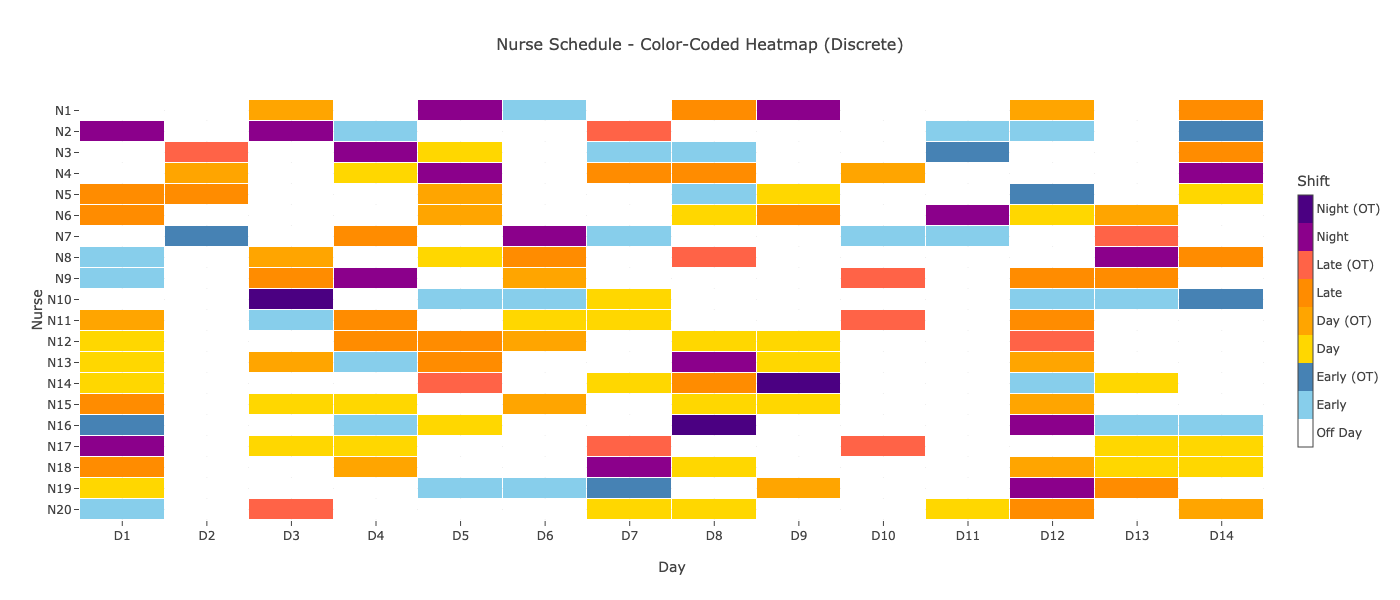
\includegraphics[width=0.9\columnwidth]{SDM-F.png}
\caption{Schedule for SDM-FATIGUE (feasible).}
\label{fig:sdm_fatigue}
\end{figure}

\begin{figure}[htbp]
\centering
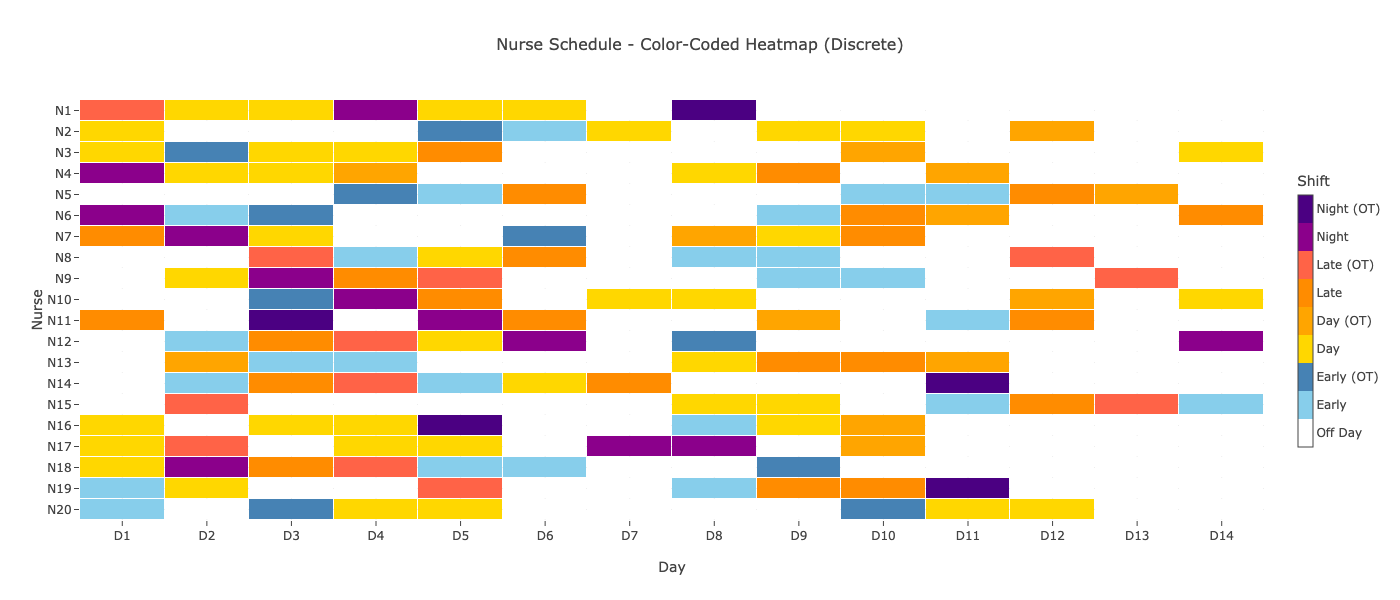
\includegraphics[width=0.9\columnwidth]{SDM-N.png}
\caption{Schedule for SDM-NO FATIGUE (feasible).}
\label{fig:sdm_nofatigue}
\end{figure}

\begin{figure}[htbp]
\centering
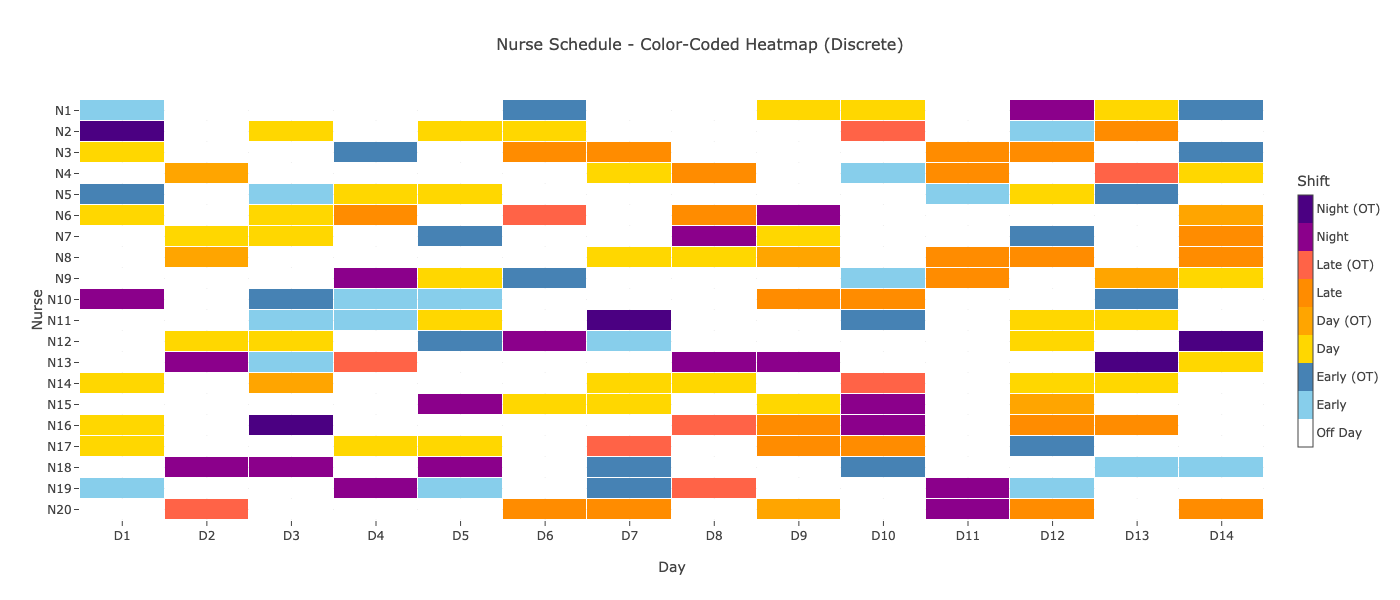
\includegraphics[width=0.9\columnwidth]{CVaR-F.png}
\caption{Schedule for CVAR-FATIGUE (feasible).}
\label{fig:cvar_fatigue}
\end{figure}

\begin{figure}[htbp]
\centering
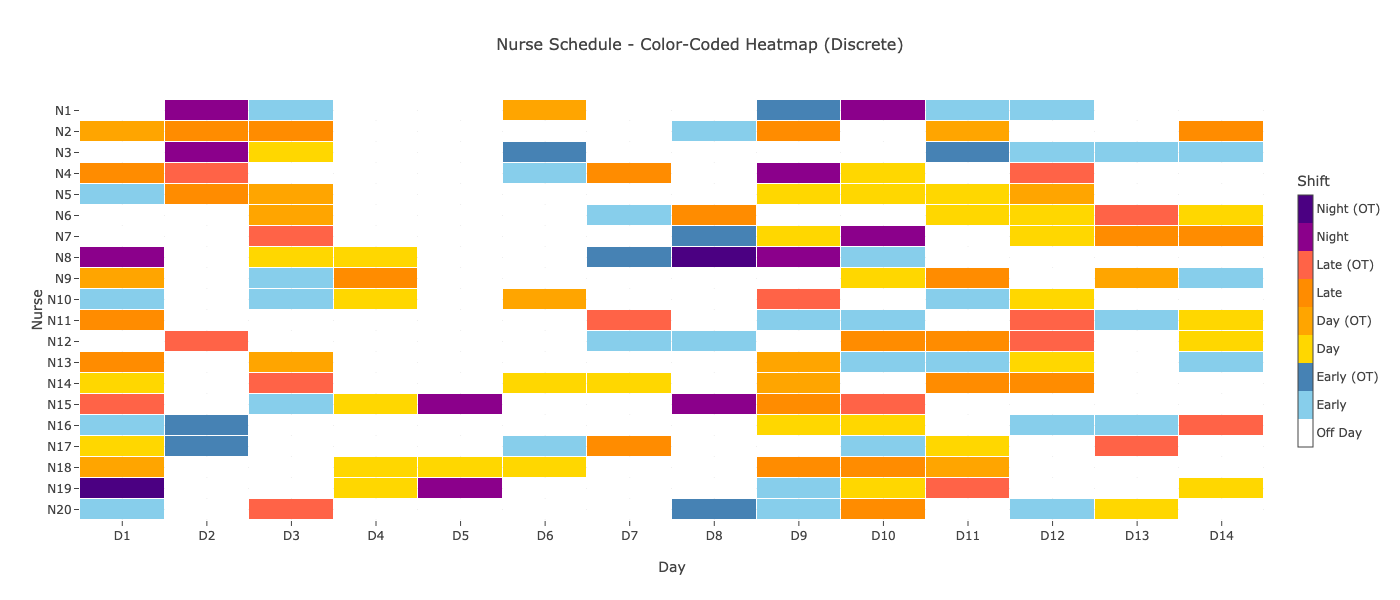
\includegraphics[width=0.9\columnwidth]{CVaR-N.png}
\caption{Schedule for CVAR-NO FATIGUE (feasible).}
\label{fig:cvar_nofatigue}
\end{figure}

\newpage
\section{Conclusion and Recommendations}
This study presented the FROST-NS framework, an integrated approach to nurse scheduling that simultaneously addresses stochastic patient demand, workforce fatigue, and operational risk. By formulating the problem as a two-stage stochastic program with Conditional Value-at-Risk (CVaR) constraints, we demonstrated the feasibility of balancing cost efficiency with robust safety standards.

The computational results highlighted significant trade-offs between operational costs and nurse well-being. Specifically, the inclusion of fatigue constraints resulted in an approximately 12\% increase in the objective value compared to the baseline model. This premium reflects the necessary investment in patient safety and staff welfare, quantifying the hidden costs often ignored in deterministic scheduling. Furthermore, the analysis revealed the critical impact of resource limitations on risk mitigation; the strict CVaR targets ($\mu=50$) proved infeasible with the current workforce of 20 nurses, underscoring that robust protection against worst-case demand surges requires commensurate staffing levels.

Comparing the experimental cases, the CVAR-FATIGUE configuration offered the most comprehensive protection but at the highest computational and operational cost. In contrast, the standard deterministic models (SDM), while computationally efficient, failed to provide guarantees against extreme understaffing events. The results suggest that for the examined parameters, satisfying strict risk criteria requires either an expansion of the nurse pool (adding 2-5 nurses) or a strategic relaxation of service level guarantees. Future implementations should focus on calibrating these risk thresholds to align with specific organizational capacities.

% \end{small}
% \end{multicols}
\clearpage
% ============================================================================
% SECTION: REFERENCES
% ============================================================================
\section{References}
\begin{itemize}[leftmargin=*]
\item [1] Meredith P, Saville C, Chiara Dall'Ora, Weeks T, Wierzbicki S, Griffiths P. Estimating Nurse Workload Using a Predictive Model From Routine Hospital Data: Algorithm Development and Validation. JMIR Medical Informatics. 2025;13:e71666-e71666. doi:https://doi.org/10.2196/71666
\item [2] Moreno-Velásquez LF, Díaz-Serna FJ, Morillo-Torre D. Dynamic multicriteria optimization for the nurse scheduling problem. Decision Science Letters. 2025;14(2):457-472. doi:https://doi.org/10.5267/j.dsl.2024.12.009
\item [3] Aristeidis Mystakidis, Christos Koukaras, Paraskevas Koukaras, Konstantinos Kaparis, Stavrinides SG, Christos Tjortjis. Optimizing Nurse Rostering: A Case Study Using Integer Programming to Enhance Operational Efficiency and Care Quality. Healthcare. 2024;12(24):2545-2545. doi:https://doi.org/10.3390/healthcare12242545
\item [4] Yasmine A, Yassine O, Farouk Y, Hicham C. Workload balancing for the nurse scheduling problem: A real-world case study from a French hospital. Socio-Economic Planning Sciences. 2024;95:102046. doi:https://doi.org/10.1016/j.seps.2024.102046
\item [5] Fourati Z, Smaoui S, Kamoun H. An integrated Lexicographic goal programming and dynamic satisfaction function model for effective nurse scheduling. Decision Analytics Journal. 2023;9:100349. doi:https://doi.org/10.1016/j.dajour.2023.100349
\item [6] Ceschia S, Luca Di Gaspero, Mazzaracchio V, Policante G, Schaerf A. Solving a real-world nurse rostering problem by Simulated Annealing. Operations Research for Health Care. 2023;36:100379-100379. doi:https://doi.org/10.1016/j.orhc.2023.100379
\item [7] Otero-Caicedo R, Eduardo C, Jaimes CB, Guzmán F, Andrés E, Camilo J. A preventive–reactive approach for nurse scheduling considering absenteeism and nurses' preferences. Operations Research for Health Care. 2023;38:100389-100389. doi:https://doi.org/10.1016/j.orhc.2023.100389
\item [8] Chen Z, Causmaecker PD, Dou Y. A combined mixed integer programming and deep neural network-assisted heuristics algorithm for the nurse rostering problem. Applied Soft Computing. 2022;136:109919-109919. doi:https://doi.org/10.1016/j.asoc.2022.109919
\item [9] Goh SL, Sze SN, Sabar NR, Abdullah S, Kendall G. A 2-Stage Approach for the Nurse Rostering Problem. IEEE Access. 2022;10:69591-69604. doi:https://doi.org/10.1109/access.2022.3186097
\item [10] Klyve KK, Senthooran I, Wallace M. Nurse rostering with fatigue modelling. Health Care Management Science. 2022;26(1):21-45. doi:https://doi.org/10.1007/s10729-022-09613-4
\item [11] Abayomi-Alli AA, Uzedu FO, Misra S, Abayomi-Alli OO, Arogundade OT. Hybrid Model of Genetic Algorithms and Tabu Search Memory for Nurse Scheduling Systems. \textit{International Journal of Service Science, Management, Engineering, and Technology}. 2022;13(1):1–20. Available from: \url{https://www.sciencedirect.com/science/article/pii/S1947959X22000122}
\item [12] Nobil AH, Sharifnia SME, Cárdenas-Barrón LE. Mixed integer linear programming problem for personnel multi-day shift scheduling: A case study in an Iran hospital. Alexandria Engineering Journal. 2022;61(1):419-426. doi:https://doi.org/10.1016/j.aej.2021.06.030
\item [13] Abadi MQH, Rahmati S, Sharifi A, Ahmadi M. HSSAGA: Designation and scheduling of nurses for taking care of COVID-19 patients using novel method of Hybrid Salp Swarm Algorithm and Genetic Algorithm. Applied Soft Computing. 2021;108:107449. doi:https://doi.org/10.1016/j.asoc.2021.107449
\item [14] Petter Strandmark, Qu Y, Curtois T. First-order linear programming in a column generation-based heuristic approach to the nurse rostering problem. Computers \& Operations Research. 2020;120:104945-104945. doi:https://doi.org/10.1016/j.cor.2020.104945
\item [15] Legrain A, Omer J, Rosat S. An online stochastic algorithm for a dynamic nurse scheduling problem. European Journal of Operational Research. 2020;285(1):196-210. doi:https://doi.org/10.1016/j.ejor.2018.09.027
\item [16] He F, Chaussalet T, Qu R. Controlling understaffing with conditional Value-at-Risk constraint for an integrated nurse scheduling problem under patient demand uncertainty. Operations Research Perspectives. 2019;6:100119. doi:https://doi.org/10.1016/j.orp.2019.100119
\item [17] Legrain A, Omer J, Rosat S. A rotation-based branch-and-price approach for the nurse scheduling problem. Mathematical Programming Computation. 2019;12(3):417-450. doi:https://doi.org/10.1007/s12532-019-00172-4
\item [18] Schoenfelder J, Bretthauer KM, Wright PD, Coe E. Nurse scheduling with quick-response methods: Improving hospital performance, nurse workload, and patient experience. European Journal of Operational Research. 2019;283(1):390-403. doi:https://doi.org/10.1016/j.ejor.2019.10.047
\item [19] Zanda S, Zuddas P, Seatzu C. Long term nurse scheduling via a decision support system based on linear integer programming: A case study at the University Hospital in Cagliari. Computers \& Industrial Engineering. 2018;126:337-347. doi:https://doi.org/10.1016/j.cie.2018.09.027
\item [20] Rahimian E, Kerem Akartunalı, Levine J. A hybrid Integer Programming and Variable Neighbourhood Search algorithm to solve Nurse Rostering Problems. European Journal of Operational Research. 2016;258(2):411-423. doi:https://doi.org/10.1016/j.ejor.2016.09.030
\item [21] Bagheri M, Devin AG, Azra Izanloo. An application of stochastic programming method for nurse scheduling problem in real word hospital. Computers \& Industrial Engineering. 2016;96:192-200. doi:https://doi.org/10.1016/j.cie.2016.02.023
\item [22] Awadallah MA, Bolaji AL, Al-Betar MA. A hybrid artificial bee colony for a nurse rostering problem. Applied Soft Computing. 2015;35:726-739. doi:https://doi.org/10.1016/j.asoc.2015.07.004
\item [23] Wu TH, Yeh JY, Lee YM. A particle swarm optimization approach with refinement procedure for nurse rostering problem. Computers \& Operations Research. 2015;54:52-63. doi:https://doi.org/10.1016/j.cor.2014.08.016
\item [24] Jafari H, Nasser Salmasi. Maximizing the nurses' preferences in nurse scheduling problem: mathematical modeling and a meta-heuristic algorithm. Journal of industrial engineering international. 2015;11(3):439-458. doi:https://doi.org/10.1007/s40092-015-0111-0
\item [25] Awadallah MA, Al-Betar MA, Khader AT, Bolaji AL, Alkoffash M. Hybridization of harmony search with hill climbing for highly constrained nurse rostering problem. Neural Computing and Applications. 2015;28(3):463-482. doi:https://doi.org/10.1007/s00521-015-2076-8
\item [26] Tassopoulos IX, Solos IP, Beligiannis GN. A two-phase adaptive variable neighborhood approach for nurse rostering. Computers \& Operations Research. 2015;60:150-169. doi:https://doi.org/10.1016/j.cor.2015.02.009
\item [27] Jafari H, Bateni S, Daneshvar P, Bateni S, Mahdioun H. Fuzzy Mathematical Modeling Approach for the Nurse Scheduling Problem: A Case Study. International Journal of Fuzzy Systems. 2015;18(2):320-332. doi:https://doi.org/10.1007/s40815-015-0051-2
\item [28] Santos HG, Toffolo M, Rafael, Ribas S. Integer programming techniques for the nurse rostering problem. Annals of Operations Research. 2014;239(1):225-251. doi:https://doi.org/10.1007/s10479-014-1594-6
\item [29] Wong TC, Xu M, Chin KS. A two-stage heuristic approach for nurse scheduling problem: A case study in an emergency department. Computers \& Operations Research. 2014;51:99-110. doi:https://doi.org/10.1016/j.cor.2014.05.019
\item [30] Hadwan M, Ayob M, Sabar NR, Qu R. A harmony search algorithm for nurse rostering problems. Information Sciences. 2013;233:126-140. doi:https://doi.org/10.1016/j.ins.2012.12.025
\item [31] Sarin SC, Sherali HD, Liao L. Minimizing conditional-value-at-risk for stochastic scheduling problems. Journal of Scheduling. 2013;17(1):5-15. doi:https://doi.org/10.1007/s10951-013-0349-6
\item [32] Jaber, M., Givi, Z., \& Neumann, W. Incorporating human fatigue and recovery into the learning–forgetting process. Applied Mathematical Modelling. 2013;37(12–13):7287–7299. doi:https://doi.org/10.1016/j.apm.2013.02.028
\end{itemize}
% \end{multicols}
\end{document}